\documentclass[../report.tex]{subfiles}

\begin{document}

\chapquote{I don't look at computers as opponents. For me, it is much more interesting to beat humans.}{Magnus Carlsen}
\chapter{Generating synthetic training data}
\label{chap:data_synthesis}

Studies in human cognition by \textcite{bilalic2010} and \textcite{zhou2018} compared skilled chess players with novices in terms of their ability to remember a chess position for a short amount of time and confirmed that highly skilled players outperform novices at this task.
Perhaps more interestingly, both studies find that skilled players remember \emph{random} positions (where pieces are positioned on random squares, not necessarily obeying the rules of chess) significantly less accurately than positions from actual chess games. 
Thus it stands to reason that in general, highly skilled chess players exhibit a more developed pattern recognition ability for chess positions than novices, but this ability is specific to positions that conform to the rules of chess and are likely to occur in actual games.

This project aims to develop a similar pattern recognition ability using machine learning, and therefore our dataset will consist of positions from real chess games. 
In doing so, we automatically ensure that the chess positions are legal and sensible.

\section{Chess positions}
\label{sec:data_chess_positions}
The positions are generated from a publicly available dataset of 2,851 games played by current World Chess Champion Magnus Carlsen \cite{64squares2020}.
We randomly select 2\% of all positions (i.e.\ configurations of chess pieces) from all games to be included in our dataset, although duplicate positions are discarded.
A total of 4,888 chess positions are obtained in this manner and saved in \gls{fen} format.

\section{Three-dimensional renders}
\label{sec:3d_renders}
In order to obtain realistic images of these chess positions, we employ a three-dimensional model of a chess set on a wooden table. 
Chess pieces are placed on the board squares according the given \gls{fen} description. 
Different camera angles and lighting setups are chosen in a random process in order to maximise diversity in the dataset.

\begin{figure}
    \centering
    \begin{tikzpicture}
        \begin{axis}[
            axis lines=middle,
            xlabel=$x$,
            ylabel=$y$,
            x=.75cm, y=.75cm,
            xmin=-4, xmax=4,
            ymin=-4, ymax=4,
            enlargelimits,
            clip=false
        ]
            \foreach \y in {-4,-2,...,2}{
                \foreach \x in {-4,-2,...,2}{
                    \edef\temp{\noexpand\fill[pattern=crosshatch, pattern color=black] (\x,\y) rectangle (1+\x,1+\y) rectangle (2+\x,2+\y);}
                    \temp
                };
            };
            \draw (-4, -4) rectangle (4, 4);
            \draw[->] (6, -1) -- (6, 1) node[above,align=center] {direction of play \\ (white)};
        \end{axis}
    \end{tikzpicture}
    \caption[The chessboard coordinate system.]{Overhead view of the coordinate system on the chessboard. The $z$-axis (not shown) points upward, normal to the chessboard surface, and the board is oriented like a chess game would be set up, i.e.\ the bottom right square is white. White's direction of play (the direction in which pawns are advanced) coincides with the $y$-axis.}
    \label{fig:cartesian_chessboard}
\end{figure}
Let us consider a three-dimensional Cartesian coordinate system whose origin lies at the centre point of the chessboard's surface, as depicted in \cref{fig:cartesian_chessboard}. 
The chessboard lies on the plane formed by the $x$ and $y$ axes, and the chess squares are of unit length. 

\paragraph{Pieces}
The pieces are positioned on the squares as dictated by the particular \gls{fen} description.
However, instead of positioning them at the centre in their respective squares, they are randomly rotated and positioned with a random offset to emulate the conditions in real chess games.
More specifically, the $x$ and $y$ position of a piece in file $i$ and rank $j$ is sampled from a bivariate normal distribution given by
\begin{equation*}
    \rvp_{i,j} \sim \normal \left(
        \begin{bmatrix}
            i \\ j
        \end{bmatrix} - \frac{7}{2},
        \frac{\mI_2}{10}
    \right).
\end{equation*}
Here, we assume that $i$ and $j$ are zero-indexed, i.e.\ the square \emph{a1} corresponds to $i=j=0$.
The reason for shifting the mean by $\frac{7}{2}$ above is that since the origin lies at the midpoint of the board, the mean must be shifted four units to the left (or downwards for the $y$-axis), but since the normal distribution should be centred on the midpoint of the square, we must add one half.
Due to the fact that the $x$ and $y$ axes are perpendicular, the two components of $\rvp$ will be independent and thus can be modelled with a covariance matrix that is a multiple of the identity matrix $\mI_2$.
Experiments showed that a variance of $\frac{1}{10}$ achieved realistic results.
Finally, the piece's rotation about its $z$-axis is sampled from a uniform distribution over the half-open interval $[0, 2\pi)$.

\paragraph{Camera}
The camera is aligned to point directly at the origin (i.e.\ the centre of the board).
It is positioned with only a small offset from the $yz$-plane to ensure that the view over the chessboard is similar to the current player's perspective. 
A slight perturbation to the $x$-component of the camera position is introduced according to a normal distribution with $\mu=0$ and $\sigma=0.8$ since the player will not usually be positioned exactly in the middle in front of the board.
An angle $\theta$ is chosen uniformly in the range $\left[\frac{\pi}{4},\frac{\pi}{3}\right]$ to represent the angle that the camera makes with the board's surface (see \cref{fig:camera_angle}) if white is to play%
\footnote{On the other hand, if it is black to play, the perspective must be from the other side of the board, so $\theta$ is chosen in the range $\left[\frac{2\pi}{3},\frac{3\pi}{4}\right]$ which is equivalent to reflecting the camera position about the $xz$-plane.}.
\begin{figure}
    \centering
    \begin{tikzpicture}
        \begin{axis}[
            % axis lines=middle,
            xlabel=$y$,
            ylabel=$z$,
            x=.5cm, y=.5cm,
            xmin=-7, xmax=7,
            ymin=0, ymax=8,
            enlargelimits
        ]
            \coordinate (cam) at (7, 7);
            \coordinate (center) at (0, 0);
            \coordinate (end) at (4, 0);
            \draw[|-|] (-4, 0) -- (4, 0) node[near start,fill=white] {board};
            \draw[->,dashed] (cam) -- (0, 0);
            \draw (cam) -- (6, 6.7) -- (6.7, 6) -- (cam) node[above] {camera};
            \pic[draw, ->, "$\theta$", angle radius=1cm] {angle = end--center--cam};
        \end{axis}
    \end{tikzpicture}
    \caption{Side view of the camera setup for the scenario where it is white to move. }
    \label{fig:camera_angle}
\end{figure}
This range is chosen because human players would typically choose a camera angle between 45 and 60 degrees to ensure maximum visibility of the pieces.
The two remaining components ($y$ and $z$) of the camera's location are then obtained using a simple trigonometric calculation such that the distance from the camera to the origin is $11$ units, a length that allows the camera to capture the entire board.

\paragraph{Lighting}
For each chess position, a random choice is made between two different lighting scenarios, each having equal probability of being employed.
\begin{enumerate}
    \item The first lighting mode tries to emulate a \emph{camera flash}.
        To do so, a spotlight is set up with the same location and orientation as the camera. 
        As a result, the scene is lit up quite well with no large shadows, as it can be seen in \cref{fig:lighting_flash_example}.
        \begin{figure}
            \centering
            \begin{subfigure}[b]{0.47\textwidth}
                \centering
                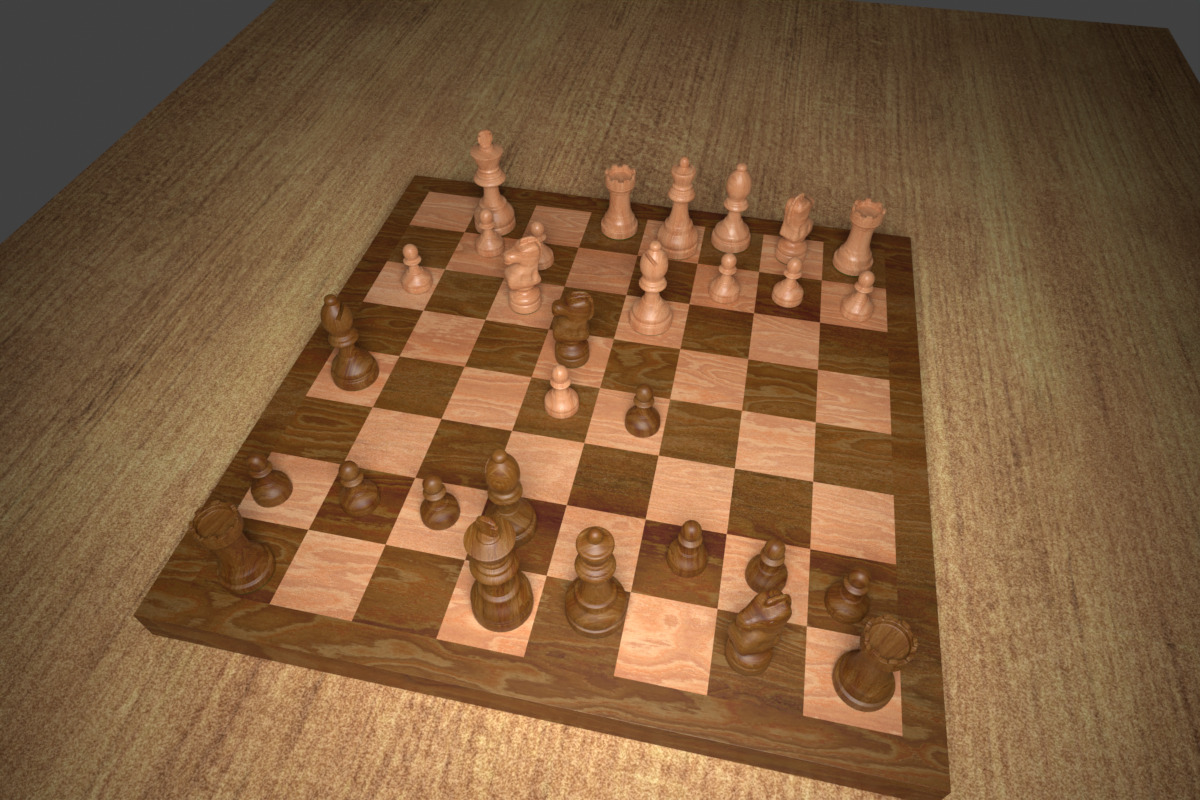
\includegraphics[width=\textwidth]{lighting_flash}
                \caption{camera flash}
                \label{fig:lighting_flash_example}
            \end{subfigure}
            \hfill
            \begin{subfigure}[b]{0.47\textwidth}
                \centering
                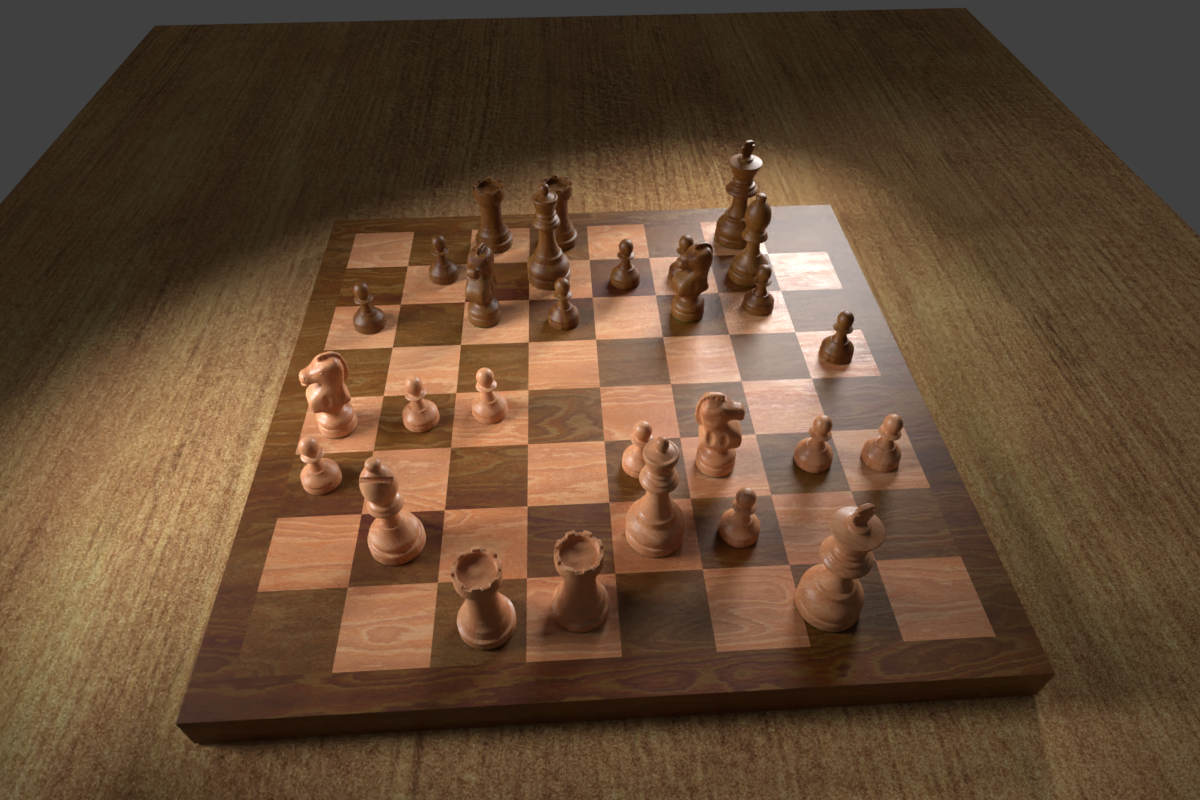
\includegraphics[width=\textwidth]{lighting_spotlights}
                \caption{spotlights}
                \label{fig:lighting_spotlights_example}
            \end{subfigure}
            \caption{Two samples from the synthesised dataset showing both types of lighting.}
            \label{fig:lighting_examples}
        \end{figure}
    \item In the other lighting mode, two spotlights are set up in the scene. 
        Their $x$ and $y$ coordinates are constrained such that they lie on a circle centred at the origin of the coordinate system with radius 10 on the $xy$-plane, as depicted in \cref{fig:chessboard_lighting_circle}, but each spotlight's location along the circumference is sampled uniformly.
        \begin{figure}
            \centering
            \begin{tikzpicture}
                \begin{axis}[
                    axis lines=middle,
                    xlabel=$x$,
                    ylabel=$y$,
                    x=.4cm, y=.4cm,
                    xmin=-10, xmax=10,
                    ymin=-10, ymax=10,
                    enlargelimits,
                    clip=false
                ]
                    \foreach \y in {-4,-2,...,2}{
                        \foreach \x in {-4,-2,...,2}{
                            \edef\temp{\noexpand\fill[pattern=crosshatch, pattern color=black] (\x,\y) rectangle (1+\x,1+\y) rectangle (2+\x,2+\y);}
                            \temp
                        };
                    };
                    \draw (-4, -4) rectangle (4, 4);

                    
                    \coordinate (o) at (0, 0);
                    \coordinate (s1) at (45:10);
                    \coordinate (s2) at (135:10);
                    \draw[dashed] (o) circle (10);
                    \draw[dashed,->] (s1) -- (o);
                    \draw[dashed,->] (s2) -- (o);

                    \draw (s1) -- (5.3, 6.3) -- (6.3, 5.3) -- cycle node[right] {spotlight 1};
                    \draw (s2) -- (-5.3, 6.3) -- (-6.3, 5.3) -- cycle node[left] {spotlight 2};
                \end{axis}
            \end{tikzpicture}
            \caption[Overhead view of the chessboard with two spotlights.]{Overhead view of the chessboard with two spotlights. The spotlights are constrained to the dashed circle such that their distance to the origin amounts to 10 units when disregarding the $z$-component.}
            \label{fig:chessboard_lighting_circle}
        \end{figure}
        Furthermore, each spotlight's $z$-component is sampled uniformly in the range $[5, 10)$.
        Finally, for each spotlight, a focus point on the chessboard surface (i.e.\ the $xy$ plane) is sampled from
        \(
            \normal\left(
                \begin{bmatrix}
                    0 \\ 0
                \end{bmatrix},
                \displaystyle \frac{5}{2} \mI_2
            \right)
        \)
        and the corresponding spotlight is rotated such that it points in that direction.
        Consequently, there is greater variabililty in the lighting because the spotlights might point at different areas on the board, thus producing different types of shadows.
        \Cref{fig:lighting_spotlights_example} shows an example rendering where the lighting produced by the spotlights is poorer than the camera flash mode.
\end{enumerate}

\section{Automated labelling}
\label{sec:automated_labelling}
Apart from eliminating the need to manually set up a large number of positions on the chessboard and photographing them, the use of a 3D model for synthetic data generation exhibits another major advantage: we can compute the required labels for the data without human intervention.
In fact, manually labelling the data is usually the most time-consuming part of the entire process.

With each render, we export a file in \gls{json} format alongside the image file containing the following information:
\begin{itemize}
    \item the pixel coordinates of the chessboard's four corner points on the rendered image;
    \item the \gls{fen} description of the pieces on the board;
    \item the colour of the current player (white/black);
    \item pixel coordinates of each piece's bounding box on the rendered image;
    \item the position and angle of the camera (in the 3D world coordinate system); and
    \item the lighting mode as well as position, angle, and focus point of each light.
\end{itemize}
The coordinates of the chessboard's corners can be computed because we know the coordinates of the relevant meshes in the 3D world coordinate system, and we know the world-to-camera-view matrix used to render the image.
It is just a matter of performing some linear algebra to compute the corresponding 2D image coordinates.
For computing the bounding boxes of the pieces, we simply project all vertices of the corresponding meshes onto the view plane and find the minimum and maximum points in the $x$ and $y$ directions.
\Cref{fig:data_synthesis_visualisation} provides a visualisation of the automatically generated labels for one sample.
\begin{figure}
    \centering
    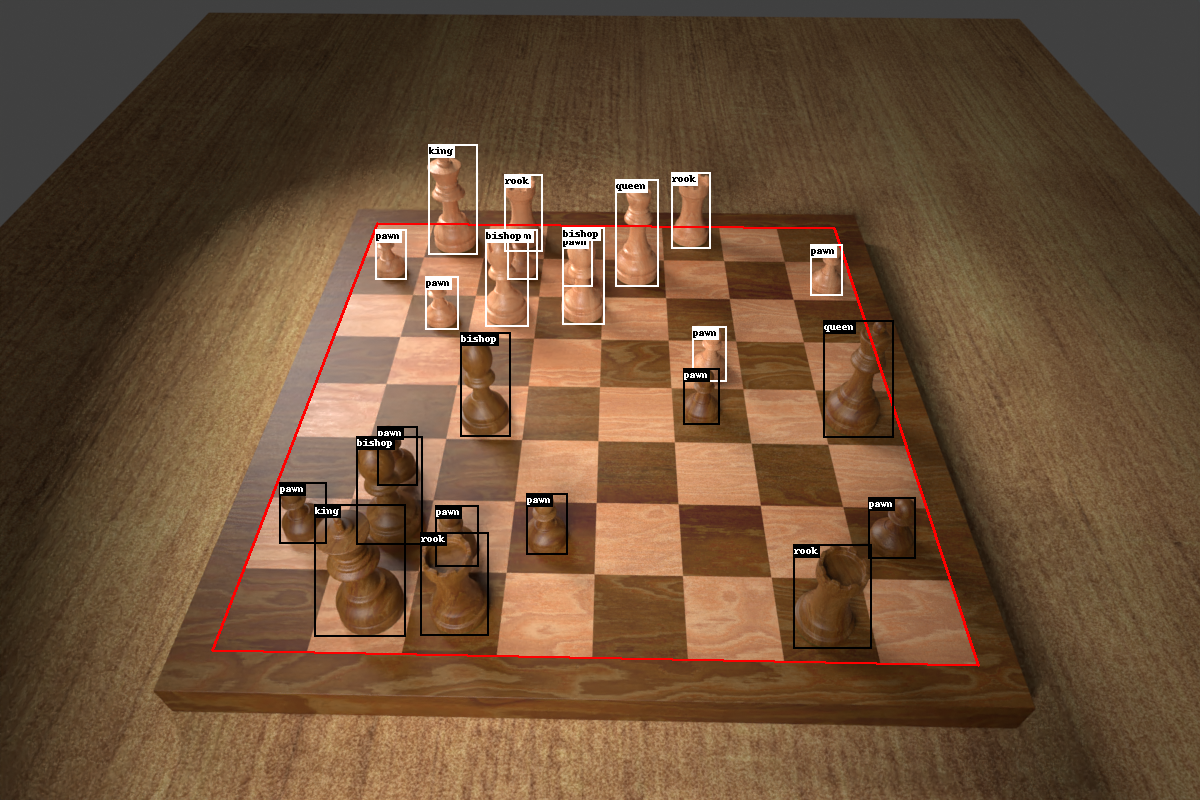
\includegraphics[width=\textwidth]{3828_data_synthesis}
    \caption[Visualisation of the automatically generated labels.]{Visualisation of the automatically generated labels. The image is rotated 90° to fit on the page. For each piece, we compute the bounding box and annotate it with the piece type. The four corners of the chessboard are joined with red lines in the visualisation.}
    \label{fig:data_synthesis_visualisation}
\end{figure}
Note that although we will not use the bounding boxes in this project, they are useful if someone should use the dataset to train an object recognition model for inferring chess positions instead of our classification-based approach.
In this project, we will mainly rely on the board's corner coordinates as well as the \gls{fen} description for training.
Furthermore, the data about the cameras and lighting is useful in iteratively refining the models by analysing which conditions perform poorly and improving on them.

\section{Splitting the dataset}
\label{sec:split_dataset}
In order to facilitate a fair evaluation of our chess recognition algorithm once it is completed, we immediately set aside 7\% of the dataset as the so-called \emph{test} set.
We will not use this data until the very end when it is time to assess the performance of our chess recognition pipeline, so we can prevent \emph{data leakage}: since we want to evaluate how our system performs on unseen data, we should not be allowed to use it during training.
A much smaller portion of the data (3\%) will be used for \emph{validation} purposes.
This subset will not directly be used for training, but for hyperparameter tuning or assessing whether a model overfits to the training data.
Finally, the remaining 90\% constitutes the training set.
\Cref{fig:dataset_split} shows the proportions of the splits, including the actual number of samples in each subset.
Note that the aforementioned splits are performed only once on the shuffled dataset and the associated \gls{json} and image files are moved into three different folders to ensure that the same split is used each time.

\begin{figure}
    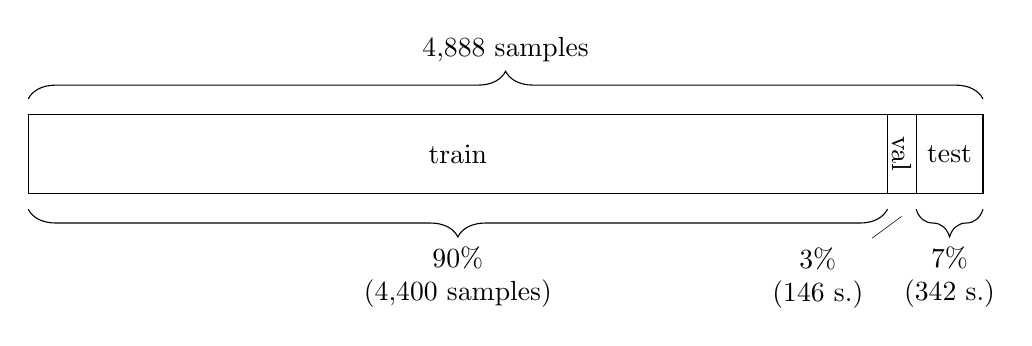
\begin{tikzpicture}
        \draw (0,0) rectangle (\textwidth,1);
        \draw (0,0) rectangle (.9\textwidth,1) node[midway] {train};
        \draw (.9\textwidth,0) rectangle (.93\textwidth,1) node[midway,rotate=-90] {val};
        \draw (.93\textwidth,0) rectangle (\textwidth,1) node[midway] {test};
        \draw [decorate,decoration={brace,amplitude=10pt}]
            (0,1.2) -- +(\textwidth,0)
            node [black,midway,above,yshift=10pt] {4,888 samples};
        \draw [decorate,decoration={brace,amplitude=10pt}]
            (.9\textwidth,-.2) -- (0,-.2)
            node [black,midway,below,yshift=-10pt,align=center] {90\%\\(4,400 samples)};
        \node[pin={[pin edge={black},align=center]-143:3\%\\(146 s.)}] at (.925\textwidth,-.2) {};
        \draw [decorate,decoration={brace,amplitude=10pt}]
            (\textwidth,-.2) -- (.93\textwidth,-.2)
            node [black,midway,below,yshift=-10pt,align=center] {7\%\\(342 s.)};
    \end{tikzpicture}
    \caption{Visual representation of the dataset split.}
    \label{fig:dataset_split}
\end{figure}

\end{document}